\chapter{检查、导出与可追溯交付}

材料学博士生小周终于把钙钛矿太阳能电池界面钝化论文的稿件投了出去。两周后，稿件没有进入同行评审，而是收到了一封来自期刊编辑部的技术退回邮件。退回理由有两条：第一，论文的 Figure 2 虽然以 PDF 格式上传，但其中的电流密度—电压（J–V）曲线与稳定性曲线在出版系统预检时被识别为低分辨率位图，而非矢量线条图；第二，面板 a 器件结构示意图中的层名文字在缩放到期刊栏宽后，字号掉到了 5 pt，低于该期刊要求的 7 pt 下限。

同一天下午，一位习惯打印读论文的合作者拿着黑白激光打印稿走进实验室，指着 Figure 2 下排的两条实线问小周：“灰度打印出来两条线深浅完全一样，哪条是对照组，哪条是钝化改性组？”紧接着，接手课题的师妹也发来消息，想把 Figure 2c 的数据重画成组会幻灯片，却发现课题组网盘里存着 \texttt{fig2\_final.png}、\texttt{fig2\_final2.pdf} 和 \texttt{fig2\_ok\_zh.png} 三个文件，谁也说不清哪一个才对应投稿版本，更找不到当时生成示意底图的提示词和修改记录。

这些问题没有一个涉及钙钛矿界面钝化本身的物理机制，却足以推迟稿件送审，并让审稿人和读者误读实验与模拟结果。一张科研图只有同时通过\textbf{印前技术检查}（有效分辨率、最终字号与线宽、矢量与容器结构、色彩与灰度可区分性）并附带\textbf{可追溯的交付档案}，才算真正完成。本章将交付前的最后一轮检查拆解为可以逐条照单执行的算式、命令与核验动作。

\section{物理尺寸、像素与有效分辨率}

在期刊投稿系统和课题组日常交流中，“这张图是不是 300 dpi”是最常被问到、也最容易产生误解的一句话。要算清分辨率，必须先把三个彼此独立的物理量区分开来：

\begin{enumerate}
\item \textbf{像素数（pixel dimensions）：}图像文件内部横向与纵向究竟包含多少个像素格，例如 $1920 \times 1080\ \text{px}$ 或 $2008 \times 1417\ \text{px}$。这是位图文件真正拥有的采样网格数量。
\item \textbf{物理尺寸（physical size）：}图片最终印在期刊页面、学位论文或海报上的实际宽度与高度，通常以毫米（mm）或英寸（$\text{in}$，$1\ \text{in} = 25.4\ \text{mm}$）计量，例如单栏宽 $85\ \text{mm}$、双栏宽 $180\ \text{mm}$ 或 $190\ \text{mm}$。
\item \textbf{有效分辨率（effective resolution）：}当这张位图被缩放到最终物理尺寸时，每英寸宽度内实际分配到多少个像素，单位写作 ppi（pixels per inch，常与印刷设备指标 dpi 混称）。
\end{enumerate}

这三个量之间只有一条换算关系（图~\ref{fig:ch13-01}）：
\begin{gather*}
\text{有效分辨率（ppi）} = \frac{\text{横向像素数（px）}}{\text{最终物理宽度（mm）} \div 25.4} \\[3pt]
\text{所需横向像素数（px）} = \frac{\text{最终物理宽度（mm）}}{25.4} \times \text{目标分辨率（dpi）}
\end{gather*}

\begin{figure}[htbp]\centering
\makebox[\linewidth][c]{% FIG ch13-01 pixels, physical size, effective resolution (Chinese)
% 栏宽按 1:2 绘制（栏宽 1 mm = 本页 0.5 mm），与英文图同一版式。
\begin{tikzpicture}[x=1mm, y=1mm, font=\sffamily\fontsize{8}{10}\selectfont, text=BookInk,
    >=Stealth]
  \tikzset{
    lbl/.style={inner sep=0pt, outer sep=0pt, anchor=south west},
    result/.style={inner sep=0pt, outer sep=0pt, anchor=north west},
    tick/.style={inner sep=0.4pt, outer sep=0pt, anchor=north},
    takeaway/.style={draw=BookTeal, line width=0.6pt, fill=white, rounded corners=1.2pt,
      inner sep=1.8mm, align=center, text width=122mm, font=\sffamily\fontsize{8}{10.5}\selectfont},
  }

  % 同一个位图文件
  \draw[BookRule, line width=0.6pt, fill=BookPale, rounded corners=1.2pt]
    (0.6, 43.0) rectangle (30.0, 76.8);
  \begin{scope}
    \clip (6.2, 63.2) rectangle (24.2, 73.325);
    \fill[white] (6.2, 63.2) rectangle (24.2, 73.325);
    \foreach \i in {0,...,15} {
      \foreach \j in {0,...,8} {
        \pgfmathparse{mod(\i+\j,2) ? 18 : 8}
        \fill[BookTeal!\pgfmathresult]
          (6.2+1.125*\i, 63.2+1.125*\j) rectangle ++(1.125, 1.125);
      }
    }
  \end{scope}
  \draw[BookRule, line width=0.4pt] (6.2, 63.2) rectangle (24.2, 73.325);
  \node[align=center, inner sep=0pt, anchor=center] at (15.3, 53.2)
    {{\fontsize{9}{11}\selectfont 文件}\\[2.5pt]1920 × 1080\,像素};

  % 两条宽度条的共同起点。85 mm -> 42.5 mm；180 mm -> 90 mm。
  \def\xO{36.2}
  \def\sS{0.5}

  \node[lbl] at (\xO, 73.4) {单栏 85\,mm};
  \fill[BookTeal] (\xO, 68.4) rectangle ({\xO+85*\sS}, 71.8);
  \node[result] at (\xO, 66.6) {1920 ÷ (85 ÷ 25.4) ≈ \textbf{574\,ppi}};

  \node[lbl] at (\xO, 56.6) {双栏 180\,mm};
  \fill[BookTeal] (\xO, 51.6) rectangle ({\xO+180*\sS}, 55.0);
  \node[result] at (\xO, 49.8) {1920 ÷ (180 ÷ 25.4) ≈ \textbf{271\,ppi}};

  \draw[BookInk, line width=0.55pt, ->] (30.0, 70.1) -- (\xO, 70.1);
  \draw[BookInk, line width=0.55pt, ->] (30.0, 53.3) -- (\xO, 53.3);

  % 与宽度条同一比例的标尺
  \draw[BookInk, line width=0.7pt] (\xO, 41.2) -- ({\xO+180*\sS}, 41.2);
  \foreach \mm/\lab in {0/0, 85/85, 180/180\,mm} {
    \draw[BookInk, line width=0.55pt] ({\xO+\mm*\sS}, 41.2) -- ({\xO+\mm*\sS}, 39.6);
    \node[tick] at ({\xO+\mm*\sS}, 39.3) {\lab};
  }
  \node[inner sep=0pt, outer sep=0pt, anchor=north west] at (0.6, 34.6)
    {同一比例尺（栏宽 1\,mm = 本页 0.5\,mm）};

  \node[takeaway, anchor=north west] at (0.6, 29.2) {%
    有效分辨率 = 像素数 ÷（宽度 mm ÷ 25.4）\\[2pt]
    改动文件里的 dpi 标签不改变像素数};
\end{tikzpicture}
}
\caption{同一文件放到不同宽度，有效分辨率不同。有效分辨率由像素数和最终印刷宽度决定，与文件中记录的 dpi 标签无关。}\label{fig:ch13-01}
\end{figure}

理解这条算式之后，两个常见的修图误区就不攻自破了。

第一个误区是\textbf{把“文件头里的 dpi 标签”当成有效分辨率}。PNG、TIFF 和 JPEG 的元数据里通常存着一个水平与垂直 dpi 数字（例如许多截图或绘图软件默认写入 72 dpi 或 96 dpi）。如果作者在图像处理软件里取消勾选“重新采样（Resample）”，只把数字从 72 改成 300，文件里的像素总数一格也没有增加；一旦排版系统把这张图拉宽到期刊双栏宽度，画面依然会因为像素不足而发虚。反过来，哪怕文件头写着 72 dpi，只要它横向有 $2126\ \text{px}$，放进 $180\ \text{mm}$ 双栏版面时的有效分辨率就是实打实的 $300\ \text{ppi}$。

第二个误区是\textbf{脱离目标版面宽度谈分辨率}。如图~\ref{fig:ch13-01} 所示，同样一张 $1920 \times 1080\ \text{px}$ 的高清位图，放进 $85\ \text{mm}$ 单栏（约 $3.35\ \text{in}$）时，有效分辨率高达 $1920 \div (85 \div 25.4) \approx 574\ \text{ppi}$，足以满足大多数期刊对照片和组合图的要求；但如果把同一文件直接拉满 $180\ \text{mm}$ 双栏（约 $7.09\ \text{in}$），有效分辨率就会立刻降到 $1920 \div (180 \div 25.4) \approx 271\ \text{ppi}$，连 $300\ \text{dpi}$ 的照片底线都达不到。同理，一张 $1024\ \text{px}$ 宽的图像放在 $85\ \text{mm}$ 单栏时约为 $306\ \text{ppi}$，一旦放到 $180\ \text{mm}$ 双栏就只剩 $144\ \text{ppi}$，肉眼即可看出明显的锯齿与模糊。

表~\ref{tab:ch13-px-calc} 给出了常见期刊栏宽与目标分辨率对应的横向像素数，以及常见图像像素宽度在不同栏宽下的有效分辨率。在新建画布或设置导出参数前，按表或公式手算一次只需十秒钟。

\begin{table}[htbp]\centering\footnotesize
\setlength{\tabcolsep}{4pt}
\renewcommand{\arraystretch}{1.18}
\caption{常见版面宽度下的目标像素数与常见像素宽度的有效分辨率换算。}\label{tab:ch13-px-calc}
\begin{tabularx}{\linewidth}{@{}>{\raggedright\arraybackslash}p{30mm}>{\raggedright\arraybackslash}p{26mm}>{\raggedright\arraybackslash}p{28mm}Y@{}}
\toprule
\textbf{计算方向} & \textbf{版面或文件参数} & \textbf{目标要求或条件} & \textbf{换算算式与结果} \\
\midrule
由宽度与 dpi 算像素 & 单栏 $85\ \text{mm}$（$3.35\ \text{in}$） & 照片 $300\ \text{dpi}$ / 组合 $600\ \text{dpi}$ & $85 \div 25.4 \times 300 \approx 1004\ \text{px}$；$\times 600 \approx 2008\ \text{px}$ \\
由宽度与 dpi 算像素 & 双栏 $180\ \text{mm}$（$7.09\ \text{in}$） & 照片 $300\ \text{dpi}$ / 组合 $600\ \text{dpi}$ & $180 \div 25.4 \times 300 \approx 2126\ \text{px}$；$\times 600 \approx 4252\ \text{px}$ \\
由宽度与 dpi 算像素 & 双栏 $190\ \text{mm}$（$7.48\ \text{in}$） & Elsevier 线条图 $1000\ \text{dpi}$ & $190 \div 25.4 \times 1000 \approx 7480\ \text{px}$（组合图 $500\ \text{dpi} \approx 3740\ \text{px}$） \\
由像素与宽度算 ppi & 横向 $1920\ \text{px}$ 文件 & 放 $85\ \text{mm}$ 单栏 / $180\ \text{mm}$ 双栏 & 单栏：$1920 \div 3.35 \approx 574\ \text{ppi}$；双栏：$1920 \div 7.09 \approx 271\ \text{ppi}$ \\
由像素与宽度算 ppi & 横向 $1024\ \text{px}$ 文件 & 放 $85\ \text{mm}$ 单栏 / $180\ \text{mm}$ 双栏 & 单栏：$1024 \div 3.35 \approx 306\ \text{ppi}$；双栏：$1024 \div 7.09 \approx 144\ \text{ppi}$ \\
\bottomrule
\end{tabularx}
\end{table}

发现手头位图的像素数不够时，很多人的第一反应是用软件把图像“插值放大”到目标像素数。图~\ref{fig:ch13-02} 用本章钙钛矿案例的模拟 J–V 曲线（目标尺寸 $85 \times 60\ \text{mm}$）展示了“低分辨率导出后插值放大”与“直接按目标分辨率输出”的对比。

\begin{figure}[htbp]\centering
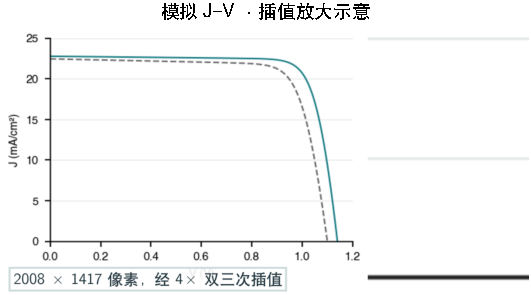
\includegraphics[width=85mm]{figures/ch13/ch13-02a-upsampled-zh.pdf}\\[1.5mm]
{\footnotesize (a) 先按 150 dpi 栅格化（$502 \times 354\ \text{px}$），再经 $4\times$ 双三次插值放大到 $2008 \times 1417\ \text{px}$}\\[3mm]
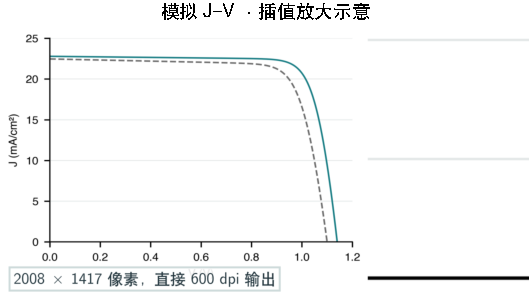
\includegraphics[width=85mm]{figures/ch13/ch13-02b-native-zh.pdf}\\[1.5mm]
{\footnotesize (b) 直接按 600 dpi 输出（$2008 \times 1417\ \text{px}$）}
\caption{像素数相同，信息量不同。(a) 150 dpi 输出后插值放大到 600 dpi；(b) 直接按 600 dpi 输出。局部为 8 倍放大。数据为模拟数据。}\label{fig:ch13-02}
\end{figure}

仔细对比图~\ref{fig:ch13-02} 的上下两幅图：两份文件的像素数完全相同，都是 $2008 \times 1417\ \text{px}$，如果只靠自动化脚本查像素尺寸，两者都会显示“达到 $600\ \text{ppi}$”。但看实际画面就能发现明显差别：在图~\ref{fig:ch13-02}a 左侧整图中，刻度数字（\texttt{0.0}–\texttt{1.2}、\texttt{0}–\texttt{25}）、纵轴标题“\texttt{J (mA/cm²)}”以及灰色虚线与青色实线都发虚发软；右侧 8 倍放大局部截取了底部黑色坐标轴线与两条浅灰水平网格线，可以看到图~\ref{fig:ch13-02}a 的黑线与网格线上下两侧都拖着一层模糊的灰边（那是 $502 \times 354\ \text{px}$ 低分辨率像素被双三次插值平滑过渡后留下的伪影），而图~\ref{fig:ch13-02}b 直接在 $600\ \text{dpi}$ 下渲染，无论左侧文字还是右侧 8 倍放大的轴线边缘都干净锐利。

顺带指出图~\ref{fig:ch13-02} 画面本身暴露出的两处排版细节：一是左下角标注像素数的白底浅框放在了固定相对坐标处，向上遮挡了横轴标题“\texttt{V (V)}”的上半截；二是右侧 8 倍放大框在纵向裁切时只保留了水平网格线与底轴，没有把右侧曲线拐点与坐标文字一起框进来。这也提醒我们，自己在做 $800\%$ 放大检查时，不要只盯着空白处的水平线，而要把放大镜移到曲线拐点、斜线段和上下标文字处逐一查看。

数学插值放大（双线性、双三次或 Lanczos）只是在相邻旧像素之间按函数关系填补平滑过渡的新像素，\textbf{只增加文件体积，不增加任何真实空间信息}。比传统插值更需要警惕的是\textbf{生成式 AI 超分辨率放大}。如果把分辨率偏低的扫描电镜（SEM）照片、荧光显微图像或蛋白印迹条带放进 AI 放大工具，模型确实会让边缘看起来变“锐利”，但这种锐利是神经网络根据训练集中看过的纹理猜出来的——它可能把原本模糊的晶界补成清晰的柱状晶粒，或者在背景噪声里画出根本不存在的微孔。正如第 8 章所强调的，原始实验图像属于观测证据，\textbf{严禁对作为科学证据的实验图像使用生成式 AI 放大或重绘}。若实验原图有效分辨率不足，合规做法只有两条：要么回到原始采集文件重新导出全分辨率原图，要么缩小该面板在组图中的物理宽度并在处理记录中如实写明原图像素数。

在使用 \scidraw{} 时需分清两类工具的处理机制：通用图像转换工具的 dpi 档位映射到固定最大像素边长，当原图像素不足时可能调用 AI 放大，因此绝不能用它给实验原图“补分辨率”；而组图工具（\sdtool{multi-panel-figure-maker}）的导出引擎严格按目标版面的物理毫米尺寸与设定 dpi 换算画布，并在导出的处理记录（\texttt{processing-log}）中如实记录每个面板的原始像素、排版毫米宽度与最终有效分辨率。

\section{在最终宽度下检查字号与线宽}

搞清楚有效分辨率之后，第二个在技术初审和同行阅读中高频翻车的指标是\textbf{最终印刷字号与线宽}。

许多研究生用 Python（Matplotlib）、R、Origin 或 PowerPoint 画图时，习惯在软件默认画布尺寸下看着屏幕调字号：屏幕上看 $10\ \text{pt}$ 的坐标轴文字清清楚楚，导出后塞进 Word 或 LaTeX 的单栏里，印出来却小得像蚂蚁。原因很简单：把宽图整体缩放到较窄的期刊栏宽时，图中所有文字的字号和线条的粗细都会按完全相同的几何比例线性缩小：
\[
\text{最终字号（pt）} = \text{作图时设定的字号（pt）} \times \frac{\text{最终版面宽度（mm）}}{\text{作图画布宽度（mm）}}
\]

我们拿两个最常见的作图场景算一笔账：
\begin{itemize}
\item \textbf{Matplotlib 默认宽画布缩放：}以第 1 章与第 5 章使用的配对比较图为例，原始脚本画布宽度为 $7.3\ \text{in}$（即 $7.3 \times 25.4 \approx 185.4\ \text{mm}$），坐标轴与标签字号设为 $10\ \text{pt}$。如果这张图按双栏 $180\ \text{mm}$ 满宽排版，最终字号是 $10 \times 180 \div 185.4 \approx 9.7\ \text{pt}$，完全合规；可一旦在定稿时决定把它改放进 $85\ \text{mm}$ 单栏（或作为双栏四面板组图的半栏面板），缩放比例就变成 $85 \div 185.4 \approx 0.458$，原本 $10\ \text{pt}$ 的文字印出来只剩 $10 \times 85 \div 185.4 \approx 4.6\ \text{pt}$（精确值 $4.58\ \text{pt}$）。这不仅低于 Elsevier 要求的最终 $7\ \text{pt}$ 和 PLOS ONE 要求的 $8\ \text{pt}$，甚至跌破了 Nature 允许的 $5\ \text{pt}$ 绝对下限。
\item \textbf{PowerPoint 宽屏画布缩放：}PowerPoint 默认 16:9 宽屏幻灯片宽度为 $33.867\ \text{cm}$（$338.7\ \text{mm}$）。不少同学喜欢在满屏幻灯片上用 $24\ \text{pt}$ 或 $18\ \text{pt}$ 画流程图，导出图片后缩放到 $85\ \text{mm}$ 单栏宽时，缩放比例约为 $85 \div 338.7 \approx 0.251$：画布上看似很大的 $24\ \text{pt}$ 文字会被缩成 $6.0\ \text{pt}$，而 $18\ \text{pt}$ 的注释则会缩成 $4.5\ \text{pt}$。
\end{itemize}

图~\ref{fig:ch13-03} 把配对比较数据（8 个模拟对象，其中 \texttt{SIM04} 从前测 18 降至后测 17）的两种做法按\textbf{实际 $85\ \text{mm}$ 物理宽度}直接印在书页上，让你不用算公式就能直观对比 $4.6\ \text{pt}$ 与 $7\ \text{pt}$ 的阅读感受。

\begin{figure}[htbp]\centering
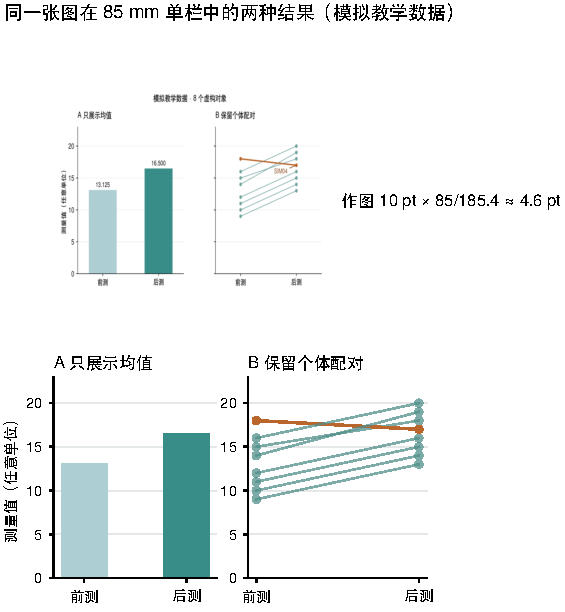
\includegraphics[width=85mm]{figures/ch13/ch13-03-text-at-final-width-zh.pdf}
\caption{同一张图在 85 mm 单栏中的两种结果。上：按 7.3 in（185 mm）宽作图、10 pt 文字，缩放后约 4.6 pt；下：按最终宽度作图，文字 7 pt。两图按实际尺寸印刷。数据为模拟教学数据。}\label{fig:ch13-03}
\end{figure}

观察图~\ref{fig:ch13-03}：上图把 $185.4\ \text{mm}$ 宽、$10\ \text{pt}$ 字号的原图缩进单栏区域，不仅纵轴标题“测量值（任意单位）”、柱顶均值（\texttt{13.125}、\texttt{16.500}）和逆向个体标签“\texttt{SIM04}”缩小到了约 $4.6\ \text{pt}$，而且由于原图贴入窄框时横向略受挤压，中文字符显得格外局促，坐标轴线与网格线也细得发飘。下图则是直接将画布宽度设为 $85\ \text{mm}$，把刻度与轴标题设为 $7\ \text{pt}$、子图标题（“\texttt{A 只展示均值}”“\texttt{B 保留个体配对}”）设为 $8\ \text{pt}$、普通个体连线设为 $0.75\ \text{pt}$、高亮个体 \texttt{SIM04} 设为 $1.2\ \text{pt}$，并删去了小尺寸下容易拥挤的柱顶三位小数，每一个汉字和数字都舒展清晰。

这里同样指出图~\ref{fig:ch13-03} 脚本生成时的一处真实版面教训：脚本原本在上下两行的右侧同一相对位置（$x = 0.76$）各写了一行边注——上行写“作图 10 pt $\times$ 85/185.4 $\approx$ 4.6 pt”，下行写“最终 7 pt”；但由于下行直接按 $85\ \text{mm}$ 满宽展开了左右两个子图（右侧子图横向延伸到了 $x = 0.98$），带白底的子图画布把下行的“最终 7 pt”边注遮挡在了底下。这再次说明，子图嵌入或图层叠加后必须肉眼核查成图，不能只看代码无报错就以为文字一定可见。

线宽遵循完全相同的缩放规律。如果在 $185\ \text{mm}$ 画布上画了一条 $0.5\ \text{pt}$ 的细线，缩到 $85\ \text{mm}$ 单栏后线宽只剩约 $0.23\ \text{pt}$；要是再缩得更小，就会逼近甚至低于期刊允许的最小线宽下限（例如 Elsevier 规定线宽应在 $0.10\text{--}1.5\ \text{pt}$ 之间），在激光打印或低倍率屏幕预览时极易出现断线。

要从根源上杜绝字号与线宽缩水，最稳妥的工作习惯只有两条：
\begin{enumerate}
\item \textbf{从一开始就按最终毫米尺寸建画布（缩放系数保持 1.0）：}单栏图直接把脚本里的 \texttt{figsize} 设为 $(85/25.4,\ H/25.4)$（或按目标期刊设为 $89\ \text{mm}$、$90\ \text{mm}$），双栏图直接设为 $(174/25.4,\ H/25.4)$（或 $183\ \text{mm}$、$190\ \text{mm}$）。这样代码里写的 $7\ \text{pt}$ 文字和 $0.75\ \text{pt}$ 线条，印在纸上就是分毫不差的 $7\ \text{pt}$ 和 $0.75\ \text{pt}$。
\item \textbf{定稿前打印一张 100\% 比例的纸质样张用尺子量：}把导出后的整图按实际毫米宽度插进一页空白文档，用普通 A4 打印机按“实际大小（100\%）”打印出来，拿直尺量一下整图宽度是否等于目标栏宽，再量一下大写英文字母或数字的高度——$1\ \text{pt} = 1/72\ \text{in} \approx 0.353\ \text{mm}$，无衬线字体（如 Arial 或 Helvetica）的大写字母高度大约是字号的 $0.7$ 倍，因此最终 $7\ \text{pt}$ 的大写字母实际高度约为 $1.7\text{--}1.8\ \text{mm}$，$8\ \text{pt}$ 约为 $2.0\ \text{mm}$。若量出来不足 $1.2\ \text{mm}$，说明某个环节发生了二次缩放，应退回脚本重出。
\end{enumerate}

\section{矢量、栅格与“容器”}

为什么小周明明上传了 \texttt{.pdf} 文件，编辑部预检系统却退回说“线条图被栅格化成了低分辨率位图”？因为他把\textbf{文件扩展名}当成了\textbf{文件内部存储的内容类型}。

在科研绘图交付中，所有的图像文件可分为三类（图~\ref{fig:ch13-04}）：
\begin{itemize}
\item \textbf{纯栅格文件（PNG、TIFF、JPEG）：}文件内部只存二维像素矩阵。放大到 $800\%$ 时，斜线、曲线和文字边缘都会露出一个个方形像素格。这类格式适合存放本来就由像素采集得到的照片、显微镜图像、电泳条带，以及由图像模型生成的无文字示意底图。
\item \textbf{真矢量内容（内含路径与文字对象的 PDF、SVG、EPS）：}文件内部用数学坐标记录直线的端点、贝塞尔曲线的控制点、多边形的填充色，以及文字的字符串与嵌入字体。无论放大到 $800\%$ 还是更高倍率，线条边缘依然锐利，图中的坐标轴标签可以用鼠标直接拖选复制。
\item \textbf{“容器”文件（只包着一张位图的 PDF、SVG、EPS、PPTX）：}PDF、SVG、EPS 和 PPTX 在技术标准上都是\textbf{复合容器格式}——它们既可以装矢量路径和字体，也可以什么矢量对象都不装，只在页面里塞一张现成的 PNG 或 JPEG 位图。如果你先把图表保存成一张 $150\ \text{dpi}$ 的 PNG，再在软件里“另存为 PDF”，得到的文件虽然顶着 \texttt{.pdf} 的扩展名，骨子里却是一张彻头彻尾的位图。
\end{itemize}

\begin{figure}[htbp]\centering
\resizebox{\linewidth}{!}{% FIG ch13-04 what's inside the file (Chinese)
\usetikzlibrary{arrows.meta,positioning,fit}
\begin{tikzpicture}[
  font=\sffamily\footnotesize, text=BookInk,
  card/.style={draw=BookRule, line width=0.6pt, rounded corners=3pt,
    fill=BookPale!30, minimum width=42mm, minimum height=38mm, align=center, inner sep=5pt},
  icon/.style={font=\scriptsize, align=center},
]
  \node[card] (C1) at (0,0) {%
    \textbf{栅格文件}\\PNG、TIFF、JPEG\\[4pt]
    \tikz{\foreach \x in {0,1,2,3} \foreach \y in {0,1,2,3}
      \fill[BookTeal!35] (\x*0.35,\y*0.35) rectangle ++(0.32,0.32);}\\[3pt]
    \scriptsize 放大后出现像素格；\\适合照片与显微图像};
  \node[card, right=6mm of C1] (C2) {%
    \textbf{矢量内容}\\PDF、SVG、EPS 内的路径与文字\\[4pt]
    \tikz{\draw[BookTeal, line width=0.8pt] (0,0.6) .. controls (0.5,1.2) and (1.2,0.2) .. (1.6,0.8);
      \node[font=\sffamily] at (0.8,0.2) {Aa};}\\[3pt]
    \scriptsize 放大后边缘仍锐利；\\文字可选中、字体已嵌入};
  \node[card, right=6mm of C2] (C3) {%
    \textbf{容器}\\扩展名像矢量，内容是位图\\[4pt]
    \tikz{\draw[BookRule, fill=white] (-0.1,-0.1) rectangle (1.7,1.3);
      \foreach \x in {0,1,2} \foreach \y in {0,1,2}
        \fill[BookInk!25] (0.2+\x*0.35,0.2+\y*0.28) rectangle ++(0.3,0.24);}\\[3pt]
    \scriptsize PDF/SVG/EPS/PPTX\\可能只包着一张位图};

  \node[draw=BookTeal, fill=white, rounded corners=2pt, inner sep=5pt,
    text width=132mm, align=left, font=\scriptsize, below=8mm of C2] (how) {%
    \textbf{怎么查：}\ 
    \texttt{pdffonts}（有无嵌入字体）·
    \texttt{pdfimages -list}（几张位图、多少 ppi）·
    800\,\% 放大 · SVG 搜 \texttt{<image} · PPTX 解压查看 \texttt{ppt/media/}};

  \node[draw=BookRule, fill=BookPale!15, rounded corners=2pt, inner sep=4pt,
    text width=132mm, align=left, font=\scriptsize, below=3mm of how] {%
    \textbf{SciDraw AI 中需注意的导出：}
    数据图声明式路径的 PDF/EPS 为栅格包装；
    图像转 SVG 文字层模式含位图背景；
    图像转 PPTX = 背景图 + OCR 文本框；
    组图 PPTX 面板为位图、编号为文字。};
\end{tikzpicture}
}
\caption{文件扩展名不说明内容。PDF、SVG、EPS 和 PPTX 既可以装矢量对象，也可以只包一张位图。}\label{fig:ch13-04}
\end{figure}

要判断一个 PDF、SVG 或 PPTX 里到底装的是真矢量还是“位图容器”，有五种简单直接的检验方法：

\begin{enumerate}
\item \textbf{用 \texttt{pdffonts} 检查嵌入字体（命令行）：}Poppler 工具包中的 \texttt{pdffonts} 命令会列出 PDF 内包含的所有字体及其嵌入状态（\texttt{emb=yes} 表示已嵌入，\texttt{sub=yes} 表示已子集化）。如果一张带坐标轴文字的图跑完 \texttt{pdffonts} 后一行字体都没有输出，只有两种可能：要么整张图（含文字）已被栅格化为位图，要么所有文字都被转成了曲线轮廓（outlines）。请注意，Nature 等期刊的终稿指南明确要求线条图与文字不要栅格化、也不要把文字转曲。
\item \textbf{用 \texttt{pdfimages -list} 清点内部位图（命令行）：}运行该命令会把 PDF 里包含的每一张位图都列出来，逐行报告页码、像素宽高（\texttt{width}、\texttt{height}）、色彩空间（\texttt{rgb}、\texttt{gray}、\texttt{cmyk}）以及按页面物理尺寸折算的 \texttt{x-ppi} 和 \texttt{y-ppi}。如果一张纯折线图 PDF 在 \texttt{pdfimages -list} 里出现一张覆盖全页的位图，它就是被栅格化的容器。相反，像第 9 章那种既有示意底图（面板 a、b）又有数据曲线（面板 c、d）的组合图 PDF，正常的 \texttt{pdfimages -list} 输出应当\textbf{只列出面板 a 和 b 对应的两张位图}，而面板 c 和 d 不出现在位图列表里——因为照片和模型生成底图本来就是栅格图像，放进 PDF 依然是栅格，这是完全正常的；真正不能被栅格化的是数据图与文字标签。
\item \textbf{在阅读器里放大到 800\% 并尝试选中文字（免命令行）：}用任意 PDF 阅读器打开文件，先用鼠标选择工具涂抹坐标轴文字看能否按字符选中，再把视图放大到 $800\%$，看折线拐角与字母弧线是保持平滑锐利，还是变成了马赛克阶梯；在 Adobe Acrobat Pro 中也可以使用“输出预检（Preflight）”直接查看每个对象的类型。
\item \textbf{用文本编辑器检查 SVG：}用代码编辑器打开 \texttt{.svg} 文件，搜索 \texttt{<image} 标签（例如 Base64 编码的内嵌 PNG）。如果整个文件只有外框加一大段编码字符串，说明它只是一张穿了 SVG 外衣的 PNG；真正的矢量图表 SVG 应当由成百上千条 \texttt{<path}、\texttt{<line} 和 \texttt{<text>} 标签组成。
\item \textbf{解压检查 PPTX：}将 \texttt{.pptx} 文件复制一份、改扩展名为 \texttt{.zip} 并解压，打开其中的 \texttt{ppt/media/} 文件夹，即可看到幻灯片里嵌入的所有位图文件。
\end{enumerate}

图~\ref{fig:ch13-05} 与表~\ref{tab:ch13-02} 用同一份钙钛矿模拟 J–V 数据（$85 \times 60\ \text{mm}$）展示了真矢量 PDF（\texttt{vector.pdf}）与容器 PDF（\texttt{container.pdf}）在 $800\%$ 放大下的视觉对比及实测命令输出。

\begin{figure}[htbp]\centering
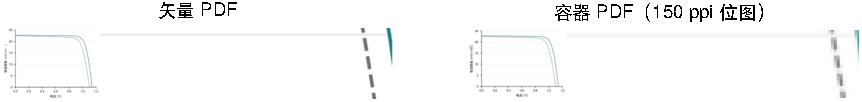
\includegraphics[width=\linewidth]{figures/ch13/ch13-05-vector-vs-container-zh.pdf}
\caption{两个都是 PDF。左：矢量对象与嵌入字体，放大后边缘锐利；右：只包着一张 150 ppi 位图，放大后出现像素格。数据为模拟数据。}\label{fig:ch13-05}
\end{figure}

\begin{table}[htbp]\centering\footnotesize
\setlength{\tabcolsep}{4pt}
\renewcommand{\arraystretch}{1.18}
\caption{对图~\ref{fig:ch13-05} 对应的两个 PDF 文件运行 \texttt{pdffonts} 与 \texttt{pdfimages -list} 的实测结果对比。}\label{tab:ch13-02}
\begin{tabularx}{\linewidth}{@{}>{\raggedright\arraybackslash}p{25mm}>{\raggedright\arraybackslash}p{22mm}Y@{}}
\toprule
\textbf{文件名与性质} & \textbf{检查命令} & \textbf{实测命令输出摘要与判读} \\
\midrule
\texttt{vector.pdf}（真矢量 PDF） & \texttt{pdffonts} & 列出 \texttt{Helvetica}（\texttt{CID TrueType}）与 \texttt{FandolHei-Regular}（\texttt{CID Type 0C}），\texttt{emb=yes}、\texttt{sub=yes}，说明中西文字体均已作为子集嵌入文件 \\
\texttt{vector.pdf}（真矢量 PDF） & \texttt{pdfimages -list} & 无任何位图条目（空白输出），证明坐标轴、网格线与两条曲线全部为纯矢量路径 \\
\texttt{container.pdf}（位图容器 PDF） & \texttt{pdffonts} & 无任何字体条目（空白输出），证明图中可见的坐标轴文字已不再是文本对象 \\
\texttt{container.pdf}（位图容器 PDF） & \texttt{pdfimages -list} & 列出第 1 页含 1 张 RGB 位图（按 150 dpi 直接封装时为 $502 \times 355\ \text{px}$、\texttt{x-ppi=150}；若经 Matplotlib \texttt{imshow} 默认 \texttt{savefig.dpi=100} 二次保存则进一步降为 $260 \times 182\ \text{px}$、\texttt{x-ppi=100}） \\
\bottomrule
\end{tabularx}
\end{table}

对照图~\ref{fig:ch13-05} 和表~\ref{tab:ch13-02}，除了可以看到左图 8 倍放大的虚线与实线边缘平滑锐利、右图 8 倍放大的曲线碎成粗糙的阶梯方格之外，这张实测图还暴露了两个在实际作图中极易踩中的隐蔽陷阱：

第一，\textbf{嵌入字体的缺字陷阱}。请仔细观察图~\ref{fig:ch13-05} 左右两张小图纵轴标题“电流密度 (\texttt{mA/cm²})”里的上标平方符号“\texttt{²}”（Unicode \texttt{U+00B2}）：因为脚本直接给整串纵轴标签指定了中文字体 \texttt{FandolHei-Regular.otf}，而该字库恰好没有收录 \texttt{U+00B2} 这个字符，结果在左边的矢量 PDF 里“\texttt{²}”直接变成了空白（显示成 \texttt{mA/cm }），而在右边的容器 PDF 里则被渲染成了一个缺字方框（俗称“豆腐块”）。这提醒我们：即便 \texttt{pdffonts} 显示 \texttt{emb=yes}，也不能省略放大肉眼核对；凡是涉及上下标（如 $\mathrm{cm^{-2}}$、$\mathrm{SnO_2}$）或特殊希腊字母（如 $\mu\mathrm{m}$）的单位，应使用数学模式（\texttt{\$\\mathrm\{mA\\,cm\^\{\{-2\}\}\}\$}）或交由字形完整的西文字体渲染。

第二，\textbf{二次封装时的静默降采样陷阱}。如表~\ref{tab:ch13-02} 最后一行所示，把一张已经按 $150\ \text{dpi}$ 渲染好的 $502 \times 354\ \text{px}$ 位图用 Matplotlib 的 \texttt{imshow} 放进新画布并调用 \texttt{savefig("container.pdf")} 时，如果忘记显式传入 \texttt{dpi} 参数，Matplotlib 会按默认的 \texttt{savefig.dpi = 100} 把画布里的位图再压缩一次，导致 PDF 内部位图进一步退化到 $260 \times 182\ \text{px}$（仅 $100\ \text{ppi}$）。只要在交付前跑一次 \texttt{pdfimages -list}，这种静默降采样一眼就能查出来。

结合前文各章，这里把 \scidraw{} 各功能模块当前导出文件的真实内部结构汇总如下，供准备终稿时核对：
\begin{itemize}
\item \textbf{科学可视化（\sdtool{sci-vis}）：}其声明式图表渲染路径导出的 PDF 与 EPS 文件属于\textbf{栅格包装容器}（内部封装的是高分辨率位图，而非可逐根拆分的矢量曲线与文字对象）。如果目标期刊强制要求数据图必须为包含嵌入字体的真矢量 PDF/EPS，作者应从 \sdtool{sci-vis} 下载校验过的数据表，用本地确定性脚本（设 \texttt{pdf.fonttype = 42}）按最终毫米尺寸输出真矢量 PDF。
\item \textbf{图像转 SVG 与图像转 PPTX：}把位图转成 SVG 时，即便选用“文字层模式”，生成的 SVG 底部仍然包含一张位图背景；转成 PPTX 时，得到的是“一张去字背景位图 + 经光学字符识别（OCR）生成的独立文本框”，并不会把画面里的细胞、晶粒或曲线自动变成带有科研语义的矢量图形。
\item \textbf{组图工具（\sdtool{multi-panel-figure-maker}）：}导出的 PPTX 文件中，各个子面板是独立位图，左上角的面板编号（\textbf{a}、\textbf{b}、\textbf{c}、\textbf{d}）是可编辑文本框，面板内部的曲线和标签则不能在 PowerPoint 里逐条拆开编辑。
\end{itemize}

\section{颜色：RGB/CMYK、灰度与色觉差异}

颜色检查要解决三个问题：文件该存什么色彩空间？打印成黑白灰阶后各组还能不能分清？对存在色觉差异的同行读者是否友好？

\subsection*{RGB 与 CMYK：保留 RGB 母版，不要盲目自行转 CMYK}

屏幕显示器靠红、绿、蓝三原色光叠加显色（RGB 加色模式，色域较宽），而纸质印刷机靠青、品红、黄、黑四色油墨叠印显色（CMYK 减色模式，色域较窄，尤其难以印出屏幕上那种高饱和度的亮绿、亮青和荧光蓝）。

早期许多作图教程会笼统建议作者“投稿前把所有图片转成 CMYK”，但这一建议早已不符合当今主流科学期刊的出版流程。如今绝大多数学术阅读发生在线上 HTML 与 PDF 版本中；查阅本章核对的三家代表性出版社官方页面（截至 2026 年 10 月 29 日），可以看到它们一致推荐或优先接受 RGB：
\begin{itemize}
\item \textbf{Nature：}明确建议作者提交 RGB 图像；期刊生产系统会在纸质印刷时自动将 RGB 转为 CMYK，同时在网络版与在线 PDF 中完整保留色彩更丰富的 RGB 原图。
\item \textbf{Elsevier：}在图件说明中写明“RGB 优先（RGB preferred）”。
\item \textbf{PLOS ONE：}作为纯在线开放获取期刊，只要求提交每通道 8 位的 RGB（或灰度）图像。
\end{itemize}

如果作者在本地用不明来源的通用印刷配置文件（ICC profile）自行把图片转成了 CMYK，不仅在线读者看到的颜色会变得暗淡发闷，一旦所选油墨配置与印厂实际设备不匹配，还会造成二次偏色。因此，正确做法是：\textbf{始终保留嵌入标准 sRGB 配置文件的 RGB 母版并优先提交 RGB；只有当目标期刊的现行作者指南明确要求提交 CMYK 文件时，才在副本上转换，并在转换后逐一核对高饱和色块是否发生了明显的色相偏移或层次并拢。}

\subsection*{灰度可读性：用感知明度 $L^*$ 检查，而不是三通道求平均}

合作者拿着黑白打印稿问小周“哪条是对照”，戳中的正是我们在第 9 章和第 12 章留下的一处真实隐患。

第 12 章在设计钙钛矿研究配色时，为了避开刺眼的红绿撞色，选用了沉稳的深灰（\texttt{\#6E6E6E}，对照组）配青色（\texttt{\#1B7F86}，改性组）。在彩色屏幕上，这两种颜色一个偏中性灰、一个偏蓝绿，感知色差（CAM02-UCS $\Delta E$）达到 $19.8$，看起来区分度相当不错。然而，当打印机或阅读器把彩色转成灰度时，人眼感受到的明暗并不是简单地把十进制 RGB 三通道加起来除以 3，而是由符合人眼光谱灵敏度的\textbf{相对亮度（luminance $Y$）与 CIE 1976 感知明度 $L^*$} 决定的。

在标准 sRGB 色彩空间中，需先将经过伽马编码的通道值还原为线性光强 $C_{\text{lin}}$，再按 Rec.~709 权重计算相对亮度：
\[
Y = 0.2126\,R_{\text{lin}} + 0.7152\,G_{\text{lin}} + 0.0722\,B_{\text{lin}}
\]
接着将 $Y$ 非线性映射为范围在 $0\text{--}100$ 之间的感知明度 $L^*$。注意到绿色通道的权重高达 $0.7152$，红色为 $0.2126$，蓝色只有 $0.0722$。我们用这套标准公式算一下本章案例与常见草稿里的四个颜色：
\begin{itemize}
\item 对照组深灰 \texttt{\#6E6E6E}（$\text{RGB} = 110, 110, 110$）：感知明度 $\mathbf{L^* = 46.4}$；
\item 改性组青色 \texttt{\#1B7F86}（$\text{RGB} = 27, 127, 134$）：虽然蓝绿醒目，但红光分量极低，折算下来感知明度 $\mathbf{L^* = 48.4}$；
\item 常见草稿红 \texttt{\#CC0000}（$\text{RGB} = 204, 0, 0$）：感知明度 $L^* = 42.5$；
\item 常见草稿绿 \texttt{\#2CA02C}（$\text{RGB} = 44, 160, 44$）：感知明度 $L^* = 57.9$。
\end{itemize}

算式直接揭示了真相：\textbf{对照组深灰（$L^* = 46.4$）与改性组青色（$L^* = 48.4$）的感知明度只差 $2.0$ 个单位，灰度下的色差 $\Delta E$ 跌到了 $2.1$！}当两条同样粗细的实线以 $L^* = 46.4$ 和 $48.4$ 印在白纸上时，任何人的肉眼都无法分辨哪条是灰、哪条是青。这就是为什么灰度检查绝不能只靠“看着颜色不一样”来拍脑袋，必须做一次真实的 $L^*$ 灰度转换。

\subsection*{色觉差异模拟与双重编码}

除了黑白打印，科研图还直接面对具有色觉差异（colour-vision deficiency, CVD）的审稿人与读者。人类视网膜包含对长波（L，偏红）、中波（M，偏绿）和短波（S，偏蓝）敏感的三类视锥细胞。根据受影响的视锥细胞类型，先天性色觉差异主要分为三类：
\begin{enumerate}
\item \textbf{红色觉异常（protan，L 视锥异常）：}包括红色弱（protanomaly）与红色盲（protanopia），对长波红光敏感度降低，不仅红绿难辨，而且纯红色在视觉上会明显变暗。
\item \textbf{绿色觉异常（deutan，M 视锥异常）：}包括绿色弱（deuteranomaly）与绿色盲（deuteranopia），是最常见的一类，红与绿在视觉上都会坍缩成相似的黄褐色或橄榄色。
\item \textbf{蓝色觉异常（tritan，S 视锥异常）：}包括蓝色弱（tritanomaly）与蓝色盲（tritanopia），较为少见，主要表现为蓝与绿、黄与紫之间的混淆。
\end{enumerate}

正如 Wong（2011）在关于科研配色的专栏中所指出的，在北欧血统人群中，通常估计约有 $8\%$ 的男性（以及约 $0.5\%$ 的女性）存在某种程度的红绿色觉差异。此外，Crameri 等人（2020）系统论证了传统彩虹色图（如 Jet）不仅会让色觉差异读者无法分辨红绿两端，还会因为本身明度梯度不均匀而在连续数据中制造出虚假的边界与伪影。

要在作图阶段检验配色在色觉差异下的表现，科学界常用基于视觉生理模型的计算机模拟算法。早期广泛使用的方法是 Brettel 等人（1997）针对完全二色视提出的 LMS 色彩空间投影模型；后来 Machado、Oliveira 与 Fernandes（2009）提出了一套基于视锥色素光谱位移理论的生理模型，将色觉异常从轻微异常三色视到完全二色视统一参数化为严重度 $0\text{--}100$，并给出了直接作用于\textbf{线性 RGB 空间}的 $3 \times 3$ 转换矩阵。

图~\ref{fig:ch13-06} 采用 Python 的 \texttt{colorspacious} 库（1.1.2 版，经核对其内部矩阵与 Machado 等人 2009 年补充材料数值一致），在最高严重度（\texttt{severity = 100}，近似完全二色视）下，对比了钙钛矿稳定性曲线三种配色方案在原图、CIE $L^*$ 灰度以及红色弱（protan）、绿色弱（deutan）、蓝色弱（tritan）五种视图下的表现，并在每个子图右上角标出了两条曲线在当前视图下的 CAM02-UCS 色差 $\Delta E$。

\begin{figure}[htbp]\centering
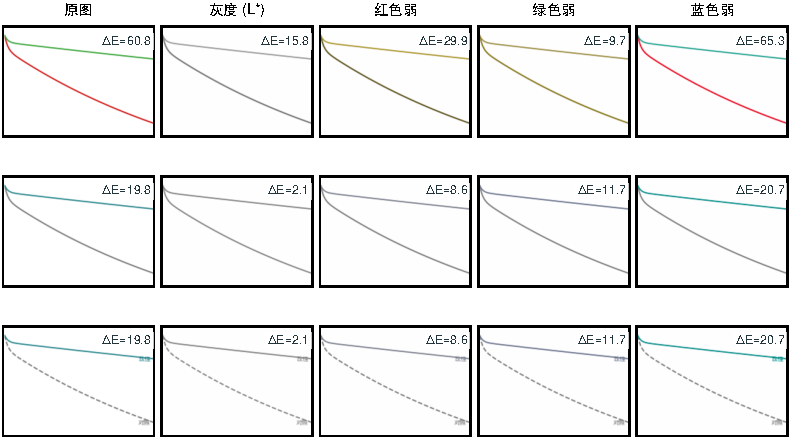
\includegraphics[width=\linewidth]{figures/ch13/ch13-06-grayscale-and-cvd-zh.pdf}
\caption{同一张图的三种配色在灰度与色觉差异模拟下的表现。第 2 行（第 12 章配色）在灰度下两组几乎无法区分；第 3 行改用线型后，在所有视图中都能区分。色觉模拟采用 Machado 等（2009）的模型，严重度 100，仅为近似。数据为模拟数据。}\label{fig:ch13-06}
\end{figure}

我们逐行核对图~\ref{fig:ch13-06} 的实测结果：
\begin{itemize}
\item \textbf{第 1 行（红 \texttt{\#CC0000} 与绿 \texttt{\#2CA02C} 实线草稿）：}在原图（$\Delta E = 60.8$）和蓝色弱（$\Delta E = 65.3$）下反差强烈；在灰度下因该红与该绿恰好有明度差（$L^*$ 分别为 $42.5$ 与 $57.9$），仍保留了 $\Delta E = 15.8$ 的深浅区别；但在最常见的绿色弱模拟（第 4 列）下，两条曲线双双变成了暗黄褐色，$\Delta E$ 骤降到 $9.7$，一旦加上图例框让读者跨空间比对颜色，极易认反。
\item \textbf{第 2 行（第 12 章初始配色：对照灰 \texttt{\#6E6E6E} 与改性青 \texttt{\#1B7F86} 均为实线）：}在红色弱（$\Delta E = 8.6$）、绿色弱（$\Delta E = 11.7$）和蓝色弱（$\Delta E = 20.7$）下尚能保持色调差异；然而一进入第 2 列的灰度（$L^*$）视图，$\Delta E$ 直接坍缩到 $\mathbf{2.1}$，上下两条实线变成了几乎完全相同的中灰色，复现了合作者拿着黑白打印稿分不清哪条是对照的场景。
\item \textbf{第 3 行（修正版：保留灰青颜色，对照组改为虚线、改性组保持实线，并在曲线右端直接标注“改性”“对照”）：}请注意，第 3 行右上角的五个颜色 $\Delta E$ 数值（$19.8$、$2.1$、$8.6$、$11.7$、$20.7$）与第 2 行分毫不差，因为我们根本没有改动两种颜色的色值；但是，由于引入了\textbf{线型（虚线对实线）}和\textbf{曲线末端直接文字标注}，即便在灰度 $\Delta E = 2.1$ 的极端情况下，任何读者也能在一秒钟内准确分清上下两条曲线。
\end{itemize}

同时，观察图~\ref{fig:ch13-06} 第 3 行的缩略图还能看到一个值得留意的细节：由于小网格缩略图里直接把 $5\ \text{pt}$ 的“改性”“对照”两个标签以垂直居中方式写在了 $t = 980\ \text{h}$ 的曲线末端坐标上，曲线本身从文字正中间穿了过去。因此，在正式制作论文终稿（如第 9 章终稿与本章交付版）时，应当把直接标注向曲线上方、下方或左侧空白处微调偏移，避免线条横穿文字笔画。

在使用任何色觉差异模拟时，必须清楚它的两条局限：第一，模拟只是针对特定理论参数的数学近似，真实个体的视锥光谱偏移程度与显示器状态各不相同，模拟通过并不等于拿到了某种绝对的“色盲无障碍认证”；第二，正如 Machado 等人（2009）在原论文中讨论的，受限于人类蓝色觉异常（tritan）的经验心理物理学数据较少，tritan 模拟矩阵的可靠性低于 protan 和 deutan。正因为如此，最稳妥的做法永远不是赌某两个颜色在所有人的眼睛里都能拉开差距，而是贯彻\textbf{双重编码（redundant encoding）}：凡是承载核心分组对比的元素，在颜色之外永远同时配上不同的线型、散点形状或直接文字标注。

\section{用 \sdtool{figure-checker} 做技术检查}

完成上述手动换算后，可以借助 \scidraw{} 的图片检查工具（即 \sdtool{figure-checker}）把与位图文件相关的技术指标做一次自动化筛查。

打开该工具上传 PNG、JPEG、WebP 或 TIFF 格式的图像后，在“图类型”中按内容选择\textbf{照片}、\textbf{混合图}或\textbf{线条图}，并在“目标版面”中选择预设的单栏（$85\ \text{mm}$）、双栏（$180\ \text{mm}$）或切换到\textbf{自定义宽度}输入精确毫米数。工具会输出六项技术检查结果与预览：(1) \textbf{有效分辨率}（按目标宽度换算；照片 $\ge 300\ \text{ppi}$、混合 $\ge 600\ \text{ppi}$、线条图 $\ge 900\ \text{ppi}$ 为“通过”，低一档为“提醒”）；(2) \textbf{文件格式}；(3) \textbf{Alpha 透明通道}（提醒去除透明背景以免排版变黑块）；(4) \textbf{色彩空间}；(5) \textbf{灰度亮度层级数与灰度预览}；(6) \textbf{三类色觉模拟下主要颜色簇是否塌缩及色觉预览}。

将报告收入交付包时，作者必须牢记五条边界——\textbf{切勿把工具界面上的“通过”当成“符合期刊全部投稿要求”}：
\begin{enumerate}
\item \textbf{它是技术检查，不是科学审核：}工具不检查统计方法、误差线定义、数据真实性或期刊特定的政策要求。
\item \textbf{默认双栏（$180\ \text{mm}$）不等于具体期刊的实际栏宽：}Nature 双栏为 $183\ \text{mm}$、Cell/Springer 为 $174\ \text{mm}$、Elsevier 为 $190\ \text{mm}$，而组图中的单个半栏面板往往只有 $84\ \text{mm}$ 或 $92\ \text{mm}$ 宽。因此检查时应改用\textbf{自定义宽度}填入真实毫米数。
\item \textbf{它不检查字号、线宽与 PDF 内部矢量结构：}一张把文字缩到 $4.5\ \text{pt}$ 的图，只要存成 $600\ \text{dpi}$ PNG，在分辨率项上照样会显示“通过”。字号与线宽须按第 13.2 节核对，PDF 内部结构须按第 13.3 节用 \texttt{pdffonts} 和 \texttt{pdfimages -list} 核对。
\item \textbf{工具内置阈值不等同于具体期刊标准：}例如工具对线条图设 $\ge 900\ \text{ppi}$ 为通过，而 Elsevier 官方指南要求线条图位图至少 $1000\ \text{dpi}$（细线 $1200\ \text{dpi}$），投稿时一律以目标期刊指南为准。
\item \textbf{自动灰度与色觉判据不能替代肉眼审视预览图：}全局灰度层级统计包含黑轴、网格和白底，未必会针对图中央两条明度相近的数据线单独报警，且快速色觉预览算法与本书图~\ref{fig:ch13-06} 采用的 Machado 矩阵结果可能略有差别，最终结论应以“点开预览图看各组是否靠线型、形状或明度清晰可分”为准。
\end{enumerate}

\section{期刊要求：以当前官方页面为准}

表~\ref{tab:ch13-01} 汇总了我们在 **2026 年 10 月 29 日** 直接打开并核对的三家出版社/期刊官方图件指南页面要点：Nature（\textit{Guide to preparing final artwork}）、PLOS ONE（\textit{Figures}）以及 Elsevier（\textit{Artwork sizing} 与 \textit{Artwork types}）。

\begin{table}[htbp]\centering\footnotesize
\setlength{\tabcolsep}{3pt}
\renewcommand{\arraystretch}{1.18}
\caption{三家期刊/出版社官方图件技术要求核对表（查阅日期：2026 年 10 月 29 日；投稿前请重新查阅目标期刊当前官方页面）。}\label{tab:ch13-01}
\begin{tabularx}{\linewidth}{@{}>{\raggedright\arraybackslash}p{18mm}YYY@{}}
\toprule
\textbf{事项} & \textbf{Nature（\textit{Guide to preparing final artwork}）} & \textbf{PLOS ONE（\textit{Figures}）} & \textbf{Elsevier（\textit{Artwork sizing / types}）} \\
\midrule
版面宽度 & 单栏 $89\ \text{mm}$；双栏 $183\ \text{mm}$；1.5 栏 $120$ 或 $136\ \text{mm}$ & 宽 $6.68\text{--}19.05\ \text{cm}$（$300\ \text{dpi}$ 下 $789\text{--}2250\ \text{px}$） & 最小 $30\ \text{mm}$；单栏 $90\ \text{mm}$；1.5 栏 $140\ \text{mm}$；双栏 $190\ \text{mm}$ \\
最大高度 & $247\ \text{mm}$ & $22.23\ \text{cm}$（$300\ \text{dpi}$ 下 $2625\ \text{px}$） & 该页面未单独列出固定最大高度 \\
分辨率要求 & 照片按印刷最大尺寸 $\ge 300\ \text{dpi}$；线条图与文字不要栅格化 & $300\text{--}600\ \text{dpi}$ & 照片 $300\ \text{dpi}$；组合图 $500\ \text{dpi}$；线条图 $1000\ \text{dpi}$（细线 $1200\ \text{dpi}$） \\
可接受格式 & AI、矢量 EPS、分层 PSD、PS、PDF、PPT、Word、Excel、CorelDraw（$\le\text{v8}$）；JPEG/TIFF/PNG 须转为 PDF/EPS/PS & TIFF 或 EPS & 线条图 EPS 或 TIFF；照片/组合图 TIFF 或最高质量 JPEG；Office 文件按混合矢量处理 \\
色彩空间 & 推荐 RGB；印刷时自动转 CMYK，在线 PDF 保留 RGB & RGB（每通道 8 bit）或灰度 & RGB 优先（RGB preferred） \\
字体与字号 & 无衬线（Helvetica 或 Arial）；面板字母 $8\ \text{pt}$ 粗体小写；其余文字最大 $7\ \text{pt}$、最小 $5\ \text{pt}$；不要转曲 & Arial、Times 或 Symbol，字号 $8\text{--}12\ \text{pt}$ & 必须嵌入字体；首选 Arial/Helvetica、Courier、Times、Symbol；正文最终 $7\ \text{pt}$，上下标 $\ge 6\ \text{pt}$ \\
其他规定 & — & 单文件 $< 10\ \text{MB}$；TIFF 去图层、无 Alpha、LZW 压缩；推荐 NAAS 预检 & 线宽保持在 $0.10\text{--}1.5\ \text{pt}$ 之间 \\
\bottomrule
\end{tabularx}
\end{table}

对比表~\ref{tab:ch13-01} 中的具体条款，有三个事实必须写进任务书：
\begin{enumerate}
\item \textbf{不同期刊的硬指标可能互相冲突：}例如 Nature 要求除面板编号（$8\ \text{pt}$）外的普通标签文字\textbf{最大不超过 $7\ \text{pt}$}（$5\text{--}7\ \text{pt}$），而 PLOS ONE 则要求图内文字在 \textbf{$8\text{--}12\ \text{pt}$} 之间。若论文换期刊重投，必须在脚本里改字号参数重新出图。
\item \textbf{同一出版社内部的不同官方指南也可能存在细微出入：}例如表~\ref{tab:ch13-01} 引用的 Nature 终稿指南规定单栏 $89\ \text{mm}$、双栏 $183\ \text{mm}$，而 Nature 旗下另一份通用图件指南文件则写着单栏 $88\ \text{mm}$、双栏 $180\ \text{mm}$，相差 $1\text{--}3\ \text{mm}$。\scidraw{} 组图工具内置期刊尺寸预设时专门记录了所依据的官方页面；投稿前仍应打开所投具体期刊当年的作者指南页复核。
\item \textbf{必须把“官方页面 URL 与查阅日期”写进任务书和交付说明：}你可以请 AI 助手帮你从指南网页摘录要点，但摘录后必须回到官方原网页逐个数字核对，并在任务书中写明查阅日期。
\end{enumerate}

\section{整理一个可追溯的交付包}

当所有图片都通过核验后，最后一步是把散落的材料整理成一个\textbf{同事无需找你问话就能独立看懂、定位和复现的交付包}。遵循科学数据管理的 FAIR 原则（Wilkinson 等，2016）与可复现计算研究十条规则（Sandve 等，2013），图~\ref{fig:ch13-08} 给出了可直接照抄的课题组级交付包标准目录树。

\begin{figure}[htbp]\centering
{\let\tag\undefined\makeatletter\tikzset{below/.code=\tikz@lib@place@handle@{#1}{north west}{0}{-1}{south west}{1}}\makeatother% FIG ch13-08 delivery package tree (Chinese)
\usetikzlibrary{positioning}
\providecommand{\ChThirteenMarkTool}{\tikz[baseline=-0.55ex]{\fill[BookInk] (0,0) rectangle (1.5mm,1.5mm);}}
\providecommand{\ChThirteenMarkSelf}{\tikz[baseline=-0.55ex]{\draw[BookInk, line width=0.35pt] (0,0) rectangle (1.5mm,1.5mm);}}
\providecommand{\tag}[1]{{\tiny\color{BookInk!75}#1}}
\noindent
\begin{tikzpicture}[
  font=\sffamily\scriptsize, text=BookInk,
  folder/.style={anchor=west, align=left},
  tagline/.style={font=\tiny, text=BookInk!75, align=left},
]
  \node[folder] (root) at (0,0) {perovskite-fig2\_\\delivery\_2026-10-29/};
  \node[folder, below=2mm of root.south west, xshift=4mm] (readme) {README.md};
  \node[tagline, below=0.5mm of readme.south west] (readmetag) {这是什么、\\怎么复现、\\联系人};
  \node[folder, below=1.5mm of readmetag.south west, xshift=4mm] (b0) {00\_brief/\\[-2pt]\tag{任务书、}\\[-1pt]\tag{期刊要求摘录}};
  \node[folder, below=1.5mm of b0.south west, xshift=4mm] (s1) {01\_source/ \ChThirteenMarkSelf\ 原图与 CSV\\[-2pt]\tag{工具 ZIP 不含}};
  \node[folder, below=1.5mm of s1.south west, xshift=4mm] (s1d) {data/ · images/};
  \node[folder, below=1.5mm of s1d.south west] (c2) {02\_code/ \ChThirteenMarkSelf\ 脚本与环境};
  \node[folder, below=1.5mm of c2.south west, xshift=4mm] (d3) {03\_drafts/ \ChThirteenMarkSelf\ v01–v04\\[-2pt]与修改指令};
  \node[folder, below=1.5mm of d3.south west, xshift=4mm] (f4) {04\_final/ \ChThirteenMarkTool\ 论文/汇报/\\[-2pt]海报终稿};
  \node[folder, below=1.5mm of f4.south west, xshift=4mm] (f4p) {paper/ · talk/ · poster/};
  \node[folder, below=1.5mm of f4p.south west] (r5) {05\_records/};
  \node[folder, below=1.5mm of r5.south west, xshift=4mm] (r5a) {ai-use-log.md \ChThirteenMarkSelf};
  \node[folder, below=1mm of r5a.south west] (r5b) {processing-log.md \ChThirteenMarkSelf};
  \node[folder, below=1mm of r5b.south west] (r5c) {checks/ \ChThirteenMarkTool\ 检查报告\\[-2pt]与命令输出};
  \node[folder, below=1mm of r5c.south west] (r5d) {multi-panel-export/ \ChThirteenMarkTool\ 组图 ZIP};

  \draw[BookInk!40, thin] (root.south west) ++(0,-1mm) coordinate (rt) -- (readme.west |- rt) -- (readme.west);
  \foreach \a/\b in {readmetag/b0,b0/s1,s1/s1d,s1d/c2,c2/d3,d3/f4,f4/f4p,f4p/r5,r5/r5a,r5a/r5b,r5b/r5c,r5c/r5d} {
    \draw[BookInk!30, thin] (\a.south west) ++(0,-0.5mm) coordinate (st) -- (\b.west |- st) -- (\b.west);
  }

  \node[tagline, anchor=north west] at ([yshift=-3mm]r5d.south-|root.west) {%
    \ChThirteenMarkTool\ 来自工具导出（组图 ZIP、\\数据下载、检查报告）\\[2pt]
    \ChThirteenMarkSelf\ 必须作者另存（原图、脚本、\\任务书、AI 使用记录）\\[4pt]
    README 三问：这是什么？\\怎么复现？\\用了哪些 AI、怎么核对的？};
\end{tikzpicture}
}
\caption{一个可被同事接手的交付包。黑色方块表示可由工具导出的内容，空心方块表示需要作者另存的材料。}\label{fig:ch13-08}
\end{figure}

图~\ref{fig:ch13-08} 用实心方块与空心方块区分了“可由工具导出的内容”和“必须由作者另存的材料”。之所以要做这个区分，是因为作者必须清楚了解当前平台上各工具的本地存储与导出边界：
\begin{itemize}
\item \textbf{组图 ZIP 不含原图与可重载工程：}组图工具导出的 ZIP 压缩包内含合成终稿（TIFF、PNG、PDF、PPTX）及处理记录（\texttt{processing-log}），但\textbf{不含未裁剪缩放的面板原始文件，也不含可跨电脑重新导入的布局文件}；组图文档只保存在当前浏览器的本地存储中，换电脑无法打开，因此 \texttt{01\_source/} 必须另存原图，\texttt{04\_final/} 保存导出成品。
\item \textbf{数据图记录源数据完整性但脚本需自存：}\sdtool{sci-vis} 会自动记录上传源数据的完整性信息（哈希值、字节数、行数）并提供数据表下载，但底层绘图代码不作为当前读者端可下载内容，因此复现脚本应保存在 \texttt{02\_code/}。
\end{itemize}

为了告别混乱命名，包内所有文件统一采用四段式命名规则：\texttt{<项目>\_<图号或用途>\_<内容>\_v<两位版本>[\_<语言>].<扩展名>}（如 \texttt{perovskite\_fig2c\_jv\_v05\_en.pdf}、\texttt{perovskite\_\allowbreak slide2b\_\allowbreak jv\_\allowbreak v02\_\allowbreak zh.png}）。执行时遵守三条纪律：(1) 只用小写 ASCII 字母、数字、连字符和下划线，不用空格或中文符号；(2) 版本号只增不改（\texttt{v01}、\texttt{v02}……），禁用 \texttt{final\_final}，日期写在交付包目录名和日志里；(3) 哪一版是“已投稿版本”在根目录 \texttt{README.md} 中唯一指明。

在 \texttt{05\_records/} 目录中，核心文档是 \textbf{AI 使用记录（\texttt{ai-use-log.md}）}与\textbf{处理记录（\texttt{processing-log.md}）}。可直接复制的 AI 使用记录模板如下：

\begin{Prompt}
# AI 使用记录 / AI-use log
项目：perovskite-passivation   图号/用途：Figure 2 / 汇报 / 海报   记录人：小周
| 日期 | 工具与功能 | 输入（版本/行数/哈希） | 实际提示词或指令路径 | 输出文件（版本） | 是否采用 | 人工核对与修改 |
|---|---|---|---|---|---|---|
| 2026-10-29 | /ai-drawing | 任务书 v1（面板 a） | 03_drafts/v01/m1_prompt.txt | m1_base_v02.png | 采用底图 | 核对 7 层顺序无误；后期叠加 7 pt 矢量层名 |
| 2026-10-29 | /ai-drawing | 任务书 v1（面板 b） | 03_drafts/v01/m2_prompt.txt | m2_sem_v01.png | 采用底图 | 确认无伪比例尺；图内左下角加“模型生成示意” |
| 2026-10-29 | /sci-vis | metrics.csv（2 行） | 03_drafts/v04/jv_instr.txt | fig2c_jv_v04.png | 部分采用 | 核对 PCE 一致；改用脚本重绘真矢量 PDF（v05） |
## 不使用 AI 的环节
数据模拟与指标计算由 02_code/sim_perovskite.py 完成；图注中的实验与模拟条件由作者撰写。
## 生成图像的证据状态
M1 为结构示意（标“不按比例”）；M2 为模型生成截面示意，非显微图像（在所有版本图内标注）。
## 期刊 AI 政策
查阅政策 URL 与日期：Elsevier AI author policy (2026-10-29)   是否需声明：按期刊要求填写。
\end{Prompt}

配套的 \texttt{processing-log.md} 则专门记录确定性处理参数：数据模拟参数与脚本版本、是否经过筛选或变换（本例无）；图像 \texttt{M1}、\texttt{M2} 的生成输入与后期缩放裁剪比例（如 \texttt{M2} 仅等比缩放、无局部修改，可直接引用组图处理记录）；以及因 P3 灰度问题修改线型的原因。

\section{完整案例：交付钙钛矿研究 Figure 2 及其衍生版本}

现在我们跟着小周把论文 Figure 2（投往执行 Elsevier 通用图件要求的期刊）、3 页组会汇报与 A0 海报走完交付全流程。

\textbf{第一步：编写交付任务书}（保存为 \texttt{00\_brief/delivery-brief.txt}）。

\begin{Prompt}
【交付对象】论文 Figure 2（四面板）；汇报第 1–3 页；A0 海报。
【目标期刊要求，查阅日期 2026-10-29】Elsevier artwork sizing / artwork types 页面：
  双栏 190 mm；正文字最终 7 pt，上下标不小于 6 pt；线宽 0.10–1.5 pt；
  线条图位图 >= 1000 dpi，组合图 >= 500 dpi，照片 >= 300 dpi；RGB 优先；嵌入字体。
【面板性质】a 示意（位图底图 + 矢量文字）；b 模型生成示意（位图）；c、d 数据图（应为真矢量）。
【检查项】有效分辨率；最终字号与线宽；c、d 为真矢量且字体嵌入；灰度与三类色觉模拟下两组可区分；图内证据标注齐全。
【不可改变】数据点（对照 PCE 19.21%、T80 约 210 h；改性 PCE 20.98%、1000 h 保留约 86%）、坐标范围、两组含义。
【交付与验收】按图 13-8 目录归档；同事只看 README 能在 10 分钟内找到 Figure 2c 的原始 CSV、生成脚本与修改指令。
\end{Prompt}

\textbf{第二步：第一轮检查结果（\texttt{v04} 初稿）。}小周对第 4 版初稿（\texttt{v04}）运行命令行检查、字号换算、CIE $L^*$ 灰度计算与 \sdtool{figure-checker} 后，发现了表~\ref{tab:ch13-case-round1} 所示的四项问题（P1–P4）。

\begin{table}[htbp]\centering\footnotesize
\setlength{\tabcolsep}{3pt}
\renewcommand{\arraystretch}{1.18}
\caption{钙钛矿研究 Figure 2 及衍生版本的第一轮交付检查结果（v04 初稿）。}\label{tab:ch13-case-round1}
\begin{tabularx}{\linewidth}{@{}c>{\raggedright\arraybackslash}p{22mm}>{\raggedright\arraybackslash}p{26mm}Y>{\raggedright\arraybackslash}p{16mm}@{}}
\toprule
\textbf{编号} & \textbf{检查项目} & \textbf{检查方法} & \textbf{实测结果与诊断} & \textbf{严重度} \\
\midrule
P1 & c、d 导出文件是否矢量 & 对从 \sdtool{sci-vis} 下载的 PDF 跑 \texttt{pdffonts}、\texttt{pdfimages -list} & 无字体条目、内含 1 张位图，属于栅格包装容器 & 高 \\
P2 & a 面板标签字号 & 把 a 源图（按 $7.3\ \text{in}$ 宽、$10\ \text{pt}$ 作图）缩进 $190\ \text{mm}$ 双栏的半栏（约 $92\ \text{mm}$） & $10 \times 92 \div 185.4 \approx 5.0\ \text{pt}$，低于 Elsevier 要求的 $7\ \text{pt}$ & 高 \\
P3 & 灰度可区分性 & 计算 CIE $L^*$：对照 \texttt{\#6E6E6E} $= 46.4$，改性 \texttt{\#1B7F86} $= 48.4$ & 两条实线在灰度下 $\Delta E = 2.1$，黑白打印几乎无法区分 & 中 \\
P4 & 位图有效分辨率 & b 面板（$1536 \times 1024\ \text{px}$）放 $92\ \text{mm}$ 宽（或 $174\ \text{mm}$ 版式的 $69\ \text{mm}$ 宽） & $1536 \div (92 \div 25.4) \approx 424\ \text{ppi}$（$69\ \text{mm}$ 时 $565\ \text{ppi}$）；a 底图（$1586 \times 992\ \text{px}$）在 $92\ \text{mm}$ 时为 $438\ \text{ppi}$。按照片类 $\ge 300\ \text{dpi}$ 满足，记录于交付说明 & 低 \\
P5 & 证据标注 & 逐图查看论文、汇报、海报 & 汇报第 2、3 页和海报均有“模拟数据”；论文 b、汇报备用页和海报均有“模型生成示意，非显微图像” & 通过 \\
\bottomrule
\end{tabularx}
\end{table}

\textbf{第三步：开具修改指令（\texttt{v04} $\rightarrow$ \texttt{v05}）。}

针对 \textbf{P1}，若在 \sdtool{sci-vis} 历史会话中确认导出格式，可输入：
\begin{Prompt}
保持数据、坐标范围、颜色和全部标注不变。我需要可编辑矢量版本用于期刊排版：
请说明当前可以导出的格式中，哪些包含矢量路径和可编辑文字。
\end{Prompt}
确认声明式路径导出的 PDF 为栅格容器后，小周改用 \texttt{02\_code/} 中的 Matplotlib 脚本读取同一份 CSV 数据（设 \texttt{pdf.fonttype = 42}）按最终物理尺寸重绘真矢量 PDF，并在处理记录中写明：“c、d 面板由脚本重绘以获得矢量文件；数值与 \sdtool{sci-vis} 版本及 \texttt{metrics.csv} 逐点核对一致。”

针对 \textbf{P2}（重绘 a 面板标签，不重新生成底图）：
\begin{Prompt}
保留 a 面板底图（v04）不变。在矢量叠加层中把所有层名改为 7 pt（最终 92 mm 宽时），
字体 Arial/Helvetica（或 TeX Gyre Heros），嵌入字体；标签与层的对应关系不变。
\end{Prompt}

针对 \textbf{P3}（数据图配色与线型双重编码）：
\begin{Prompt}
保持全部数据点、坐标、标注文字不变。对照组改为虚线（线宽 1.0 pt，颜色 #6E6E6E），
改性组保持实线 #1B7F86（1.0 pt）。面板 d 的 80% 参考线改为细点线。保留曲线末端的直接标注并避开线条。
\end{Prompt}
这一灰度问题正是在本章交付检查计算 CIE $L^*$ 时才被发现的。发现后，我们将“对照虚线、改性实线、80\% 参考线点线”回写到了第 9 章与第 12 章的终稿中，从而保证全书各章终稿与交付包中的 \texttt{v05} 版本完全一致。

\textbf{第四步：第二轮复查、终稿图注与交接验收。}复查修订后的 \texttt{v05} 确认：论文版 PDF 的 \texttt{pdffonts} 显示全部字体已嵌入，\texttt{pdfimages -list} 仅含 a、b 两张底图位图（若投稿系统要求位图 TIFF，则按线条图 $1000\ \text{dpi}$ 要求导出 $190\ \text{mm} \rightarrow 7480\ \text{px}$ 宽的 LZW 压缩 RGB TIFF）；汇报幻灯片 PNG 为 $1920 \times 1080\ \text{px}$；海报 A0 PDF 字体全部嵌入，\texttt{pdfimages -list} 仅列出 M1（$2129 \times 1332\ \text{px}$、$150\ \text{ppi}$）与 M2（$1063 \times 709\ \text{px}$、$150\ \text{ppi}$）两张位图。更新后的论文图注终稿如下：

\begin{BookNote}
\textbf{图 2}\quad 界面钝化对模拟器件性能与稳定性的影响（模拟教学数据）。(a) n-i-p 器件结构示意，不按比例。(b) 截面图样，为模型生成示意，非显微图像。(c) 模拟反向扫描 J–V 曲线（单二极管模型，AM1.5G，$100\ \text{mW\,cm}^{-2}$），对照为虚线、改性为实线；每组一条代表性曲线。(d) 归一化 PCE 随时间变化（模拟），细点线为初始值的 80\%（参考线用点线，以免与对照组的虚线混淆）。\\[3pt]
\textbf{Figure 2}\quad Effect of interfacial passivation on simulated device performance and stability (simulated teaching data). (a) Schematic of the n-i-p stack, not to scale. (b) Cross-section, model-generated illustration, not a micrograph. (c) Simulated reverse-scan J–V curves (single-diode model, AM1.5G, $100\ \text{mW\,cm}^{-2}$); control dashed, modified solid; one representative curve per group. (d) Normalized PCE over time (simulated); the thin dotted line marks 80\% of the initial value.
\end{BookNote}

最后，未参与作图的师妹仅阅读根目录下的 \texttt{README.md}，在 6 分钟内顺利找到原始数据表（\texttt{01\_source/data/}）、模拟与绘图脚本（\texttt{02\_code/}）以及第 4 版修改指令（\texttt{03\_drafts/v04/}），重跑脚本验证两组 PCE（$19.21\%$ 与 $20.98\%$）与指标表完全一致，顺利完成交接验收。

\section{AI 在这一步能做什么与不能做什么}

印前检查、格式导出与交付环节中 AI 与作者的职责边界汇总于表~\ref{tab:ch13-03}。

\begin{table}[htbp]\centering\footnotesize
\setlength{\tabcolsep}{3pt}
\renewcommand{\arraystretch}{1.18}
\caption{检查、导出与交付环节中 AI 能做什么、不能做什么与作者必须核对的内容。}\label{tab:ch13-03}
\begin{tabularx}{\linewidth}{@{}>{\raggedright\arraybackslash}p{18mm}YYY@{}}
\toprule
\textbf{环节} & \textbf{AI 能做} & \textbf{AI 不能做} & \textbf{作者要核对} \\
\midrule
尺寸与分辨率 & \sdtool{figure-checker} 按目标宽度换算有效分辨率；组图导出按真实尺寸换算 & 用放大“补回”原始图像缺失的信息；替你决定图该放单栏还是双栏 & 像素 $\div$ 最终宽度的算式；证据图像不经 AI 放大 \\
字号与线宽 & 按指令重绘数据图、调整字号 & 保证最终版面中的实际字号；知道排版时会被缩放多少 & 按最终宽度作图；100\% 样张实测 \\
文件格式 & 导出多种格式；把位图转成 SVG/PPTX 以便编辑 & 保证导出的 PDF/SVG 是带科研语义的矢量对象 & \texttt{pdffonts}、\texttt{pdfimages}、800\% 放大检查；如实标注哪些是位图 \\
颜色 & 提供灰度与三类色觉预览；建议替代配色 & 代表所有色觉差异读者的真实感受；判断颜色语义是否与全文一致 & 不只靠颜色编码；与第 4 章视觉规范一致 \\
期刊要求 & 帮你从指南页摘录要点；组图工具提供期刊预设 & 保证摘录与期刊当前页面一致 & 打开官方页面逐条核对，写明查阅日期 \\
交付记录 & 起草 \texttt{README} 与图注；组图导出处理记录；数据图记录源数据完整性 & 自动保存原图、脚本、任务书与完整的 AI 使用过程 & 交付包由同事实际试用；AI 使用记录逐行对应文件 \\
\bottomrule
\end{tabularx}
\end{table}

\section{本章检查清单}

\begin{itemize}
\item 每个位图文件：像素数、最终宽度、有效分辨率算式写在交付说明中。
\item 按最终尺寸打印 100\% 样张，用尺子量宽度，确认最小字号与线宽符合目标期刊。
\item 数据图与文字为矢量；\texttt{pdffonts} 有嵌入字体，\texttt{pdfimages -list} 只列出应为位图的面板。
\item 没有对实验图像做插值或 AI 放大；如有缩放，记录比例与方法。
\item 保留 RGB 母版（嵌入 sRGB）；只有期刊要求时才转 CMYK，并检查转换后的颜色。
\item 灰度与三类色觉模拟下各组仍可区分；关键区分不只依赖颜色。
\item \sdtool{figure-checker} 报告已保存，并把“它没有检查的项”另行核对。
\item 期刊要求来自官方页面，写有 URL 和查阅日期。
\item 交付包含原始材料、最终图、图注、AI 使用记录、处理记录与 \texttt{README}；命名规则一致。
\item 一位未参与的同事按 \texttt{README} 成功找到并复现一张图。
\end{itemize}

\section{练习}

\begin{enumerate}
\item \textbf{（算与查）}你有一张 $2400 \times 1600\ \text{px}$ 的显微图像和一张 $7\ \text{in}$ 宽、$9\ \text{pt}$ 文字的 Matplotlib 曲线图，目标期刊双栏 $183\ \text{mm}$、单栏 $89\ \text{mm}$。(a) 显微图放单栏、双栏时有效分辨率各多少？(b) 曲线图放单栏时文字多大？（参考答案：(a) $2400 \div (89 \div 25.4) \approx 685\ \text{ppi}$；$2400 \div (183 \div 25.4) \approx 333\ \text{ppi}$；(b) $9 \times 89 \div 177.8 \approx 4.5\ \text{pt}$——应按 $89\ \text{mm}$ 重新作图。）
\item \textbf{（拆开一个 PDF，\scidraw{} 实操）}在 \sdtool{sci-vis} 用任意数据（可用本书配对模拟数据）生成一张图，下载其可用的全部格式。对每个文件记录：是否含嵌入字体、是否含位图及其 ppi、$800\%$ 放大的样子。再把 PNG 上传到 \sdtool{figure-checker}，设置你目标期刊的实际宽度（自定义），记录报告。写一段 100 字说明：哪个文件适合投稿、理由是什么。
\item \textbf{（交接测试）}用图~\ref{fig:ch13-08} 的结构整理你自己的一张图，交给一位同学，只附 \texttt{README}。请他在 15 分钟内找到原始数据、生成脚本或 \scidraw{} 会话的修改指令，以及 AI 使用记录。记录他卡住的地方，修改 \texttt{README} 一次。
\end{enumerate}

\section*{参考文献}

\begin{itemize}
\item Brettel H, Vi\'{e}not F, Mollon JD. Computerized simulation of color appearance for dichromats. \textit{Journal of the Optical Society of America A}. 1997;14(10):2647--2655. doi:10.1364/JOSAA.14.002647
\item Crameri F, Shephard GE, Heron PJ. The misuse of colour in science communication. \textit{Nature Communications}. 2020;11:5444. doi:10.1038/s41467-020-19160-7
\item Elsevier. Artwork sizing; Artwork types. \url{https://www.elsevier.com/about/policies-and-standards/author/artwork-and-media-instructions/artwork-sizing}; \url{https://www.elsevier.com/about/policies-and-standards/author/artwork-and-media-instructions/artwork-types} (accessed 2026-10-29).
\item Machado GM, Oliveira MM, Fernandes LAF. A physiologically-based model for simulation of color vision deficiency. \textit{IEEE Transactions on Visualization and Computer Graphics}. 2009;15(6):1291--1298. doi:10.1109/TVCG.2009.113
\item Nature. Guide to preparing final artwork. \url{https://www.nature.com/documents/nature-final-artwork.pdf} (accessed 2026-10-29).
\item PLOS ONE. Figures. \url{https://journals.plos.org/plosone/s/figures} (accessed 2026-10-29).
\item Sandve GK, Nekrutenko A, Taylor J, Hovig E. Ten simple rules for reproducible computational research. \textit{PLoS Computational Biology}. 2013;9(10):e1003285. doi:10.1371/journal.pcbi.1003285
\item Smith NJ. \texttt{colorspacious}: A powerful, accurate, and easy-to-use Python library for doing colorspace conversions (version 1.1.2, MIT License). \url{https://github.com/njsmith/colorspacious}
\item Wilkinson MD, Dumontier M, Aalbersberg IJJ, Appleton G, Axton M, Baak A, et al. The FAIR Guiding Principles for scientific data management and stewardship. \textit{Scientific Data}. 2016;3:160018. doi:10.1038/sdata.2016.18
\item Wong B. Points of view: Color blindness. \textit{Nature Methods}. 2011;8(6):441. doi:10.1038/nmeth.1618
\end{itemize}

% TODO: 图 13-7（figures/ch13/ch13-07-figure-checker-report-zh.png，SciDraw AI /figure-checker 界面截图及 TikZ 叠加标签，\label{fig:ch13-07}）尚未生成，待截图补齐后插入第 13.5 节。
